\PassOptionsToPackage{utf8}{inputenc}
\documentclass{bioinfo}

\copyrightyear{2020} \pubyear{2020}

\access{Advance Access Publication Date: day month 2020}
\appnotes{Application Note}

\usepackage{here}

\begin{document}
\firstpage{1}

\subtitle{Genetic and population analysis}

\title[MPCC]{A Performant Matrix of Pearson$'$s Correlation Coefficient (MPCC) Calculations}
\author[Arends \textit{et~al}.]{
Danny Arends\,$^{\text{\sfb 1, $\dagger$}}$,
Mitch Horton\,$^{\text{\sfb 2, $\dagger$}}$,
Chad Burdyshaw\,$^{\text{\sfb 2, $\dagger$}}$,
Udit Gulati\,$^{\text{\sfb 3}}$,
Christian Fischer\,$^{\text{\sfb 4}}$,
Robert W. Williams\,$^{\text{\sfb 4}}$,
Pjotr Prins\,$^{\text{\sfb 4}}$,
Glenn Brook\,$^{\text{\sfb 2, *}}$}
\address{$^{\text{\sf 1}}$Z{\"u}chtungsbiologie und molekulare
Genetik, Albrecht Daniel Thaer-Institut, Berlin, 10115, Germany \\
$^{\text{\sf 2}}$The Joint Institute for Computational Sciences,
University of Tennessee, Oak
Ridge, TN 37830, USA\\
$^{\text{\sf 3}}$Computer Science Dept. Indian Institute of
Information Technology, Una, Himachal Pradesh, India\\
$^{\text{\sf 4}}$Genetics, Genomics and Informatics, University
of Tennessee Health Science Center, Memphis, TN 38163, USA.}

\corresp{$^\dagger$Contributed equally and should be considered
joined first authors, $^\ast$To whom correspondence should be
addressed.}

\history{Received on XXXXX; revised on XXXXX; accepted on XXXXX}

\editor{Associate Editor: XXXXXXX}

\abstract{ \textbf{Motivation:}  We present a novel
  high performance and robust matrix-based Pearson correlation
  coefficent (MPCC) algorithm that handles missing data and makes
  effective use of modern CPU Advanced Vector Extensions (AVX)
  extensions. Computation of correlations has
  common use in biomedical applications and research. With the rapidly
  growing amount of data acquired from sequencing, combined with
  growing body of phenotype data from medical and experimental
  biology, we find that computing correlations in networks of
  relations is a recurring bottleneck. Especially computations of
  correlations with incomplete data are slow. \\
\textbf{Results:} Our method is a reformulation of the
  original Pearson's correlation coeffient (PCC) algorithm where 
  the lion's share of the computation is handled by fast 
  matrix-matrix products. On a single Intel Xeon Gold 6148
  $@$ $2.4$ GHz (Skylake) CPU MPCC achieves 4.3 TFlop/s in single
  precision (i.e., $77\%$ of the theoretical peak). We show how MPCC
  outperforms the existing implementation in R by $200$ times. \\
\textbf{Availability:} Our source code is available as a C
  library for R published under a dual licence, the free and open 
  source software GPL-v3 licence as well as the 3-Clause BSD License.
  at \href{https://github.com/UTennessee-JICS/MPCC}{https://github.com/UTennessee-JICS/MPCC}\\
\textbf{Contact:} \href{glenn-brook@tennessee.edu}{glenn-brook@tennessee.edu}\\
\textbf{Supplementary
  information:} Supplementary data are available
  at \textit{Bioinformatics} online.}

\maketitle


\section{Introduction}

The use of Pearson's correlation coefficient (PCC) is ubiquitous
across all fields of biology ranging from agriculture to
zoology. Large scale computation of correlations are found in many
areas of biology and bioinformatics.  For example, genotype
correlations are used to construct haplotypes, build genetic maps, and
order markers within the genome. Pearson's correlations are also used
in co-expression analysis \citep{Tesson:2010}, (genome wide)
association analysis, reconstruction of genetic
networks \citep{Fukushima:2013}, weighted correlation network analysis
(WGCNA) \citep{Horvath:2008} and correlated trait locus (CTL)
mapping \citep{Arends2016a}.


%The mathematical formula for Pearson$'$s correlation were derived by
%Auguste Bravais in 1844. However, as Stigler's Law \citep{Stigler1980} dictates,
%the name of the method credits Karl Pearson, who was building on ideas published
%by Francis Galton in the 1880s.

\enlargethispage{12pt}

The work presented here is motivated by Genenetwork, a service for
web-based genetics \citep{Sloan2016} which routinely performs a matrix
of Pearson's Correlation Coefficient (PCC) calculations to find
relationships between and among genotypes and phenotypes in mouse and
rat strains. These calculations are a bottleneck for moderate to large
problem sizes, especially when accounting for missing data.

Consider the case where pairwise correlation is computed within the
set of phenotypes: the BxD family is a panel of 150 recombinant inbred
mice derived from parents C57BL/6J and DBA/2J. The BxD data collection
in Genenetwork consists of high-density genotypes with 7,000 classical
phenotypes and data sets containing 100,000+ gene expression
phenotypes \citep{Ashbrook:2019}.  All phenotype columns miss data and
with the default $cor()$ implementation of Pearson's correlation in
the R language for statistical computing \citep{R:2005} the function
is slow when handling missing data. It also lacks support for
multi-threading. With MPCC we implemented a full matrix method which
is a drop-in replacement for $cor()$, is multi-threaded and can handle
missing data.


% All BxD phenotype, genotype, and omics data is freely available on
% \href{https://genenetwork.org/}{GeneNetwork.org} \citep{Sloan2016}.
% GeneNetwork is an online platform for data storage and analysis,
% including Pearson's correlation.
% and performs well when no missing data is present. In the
% case of missing data, however, two strategies are used to deal with the
% missing data.


% \vspace*{-5mm}

\begin{figure}[H]
\centering
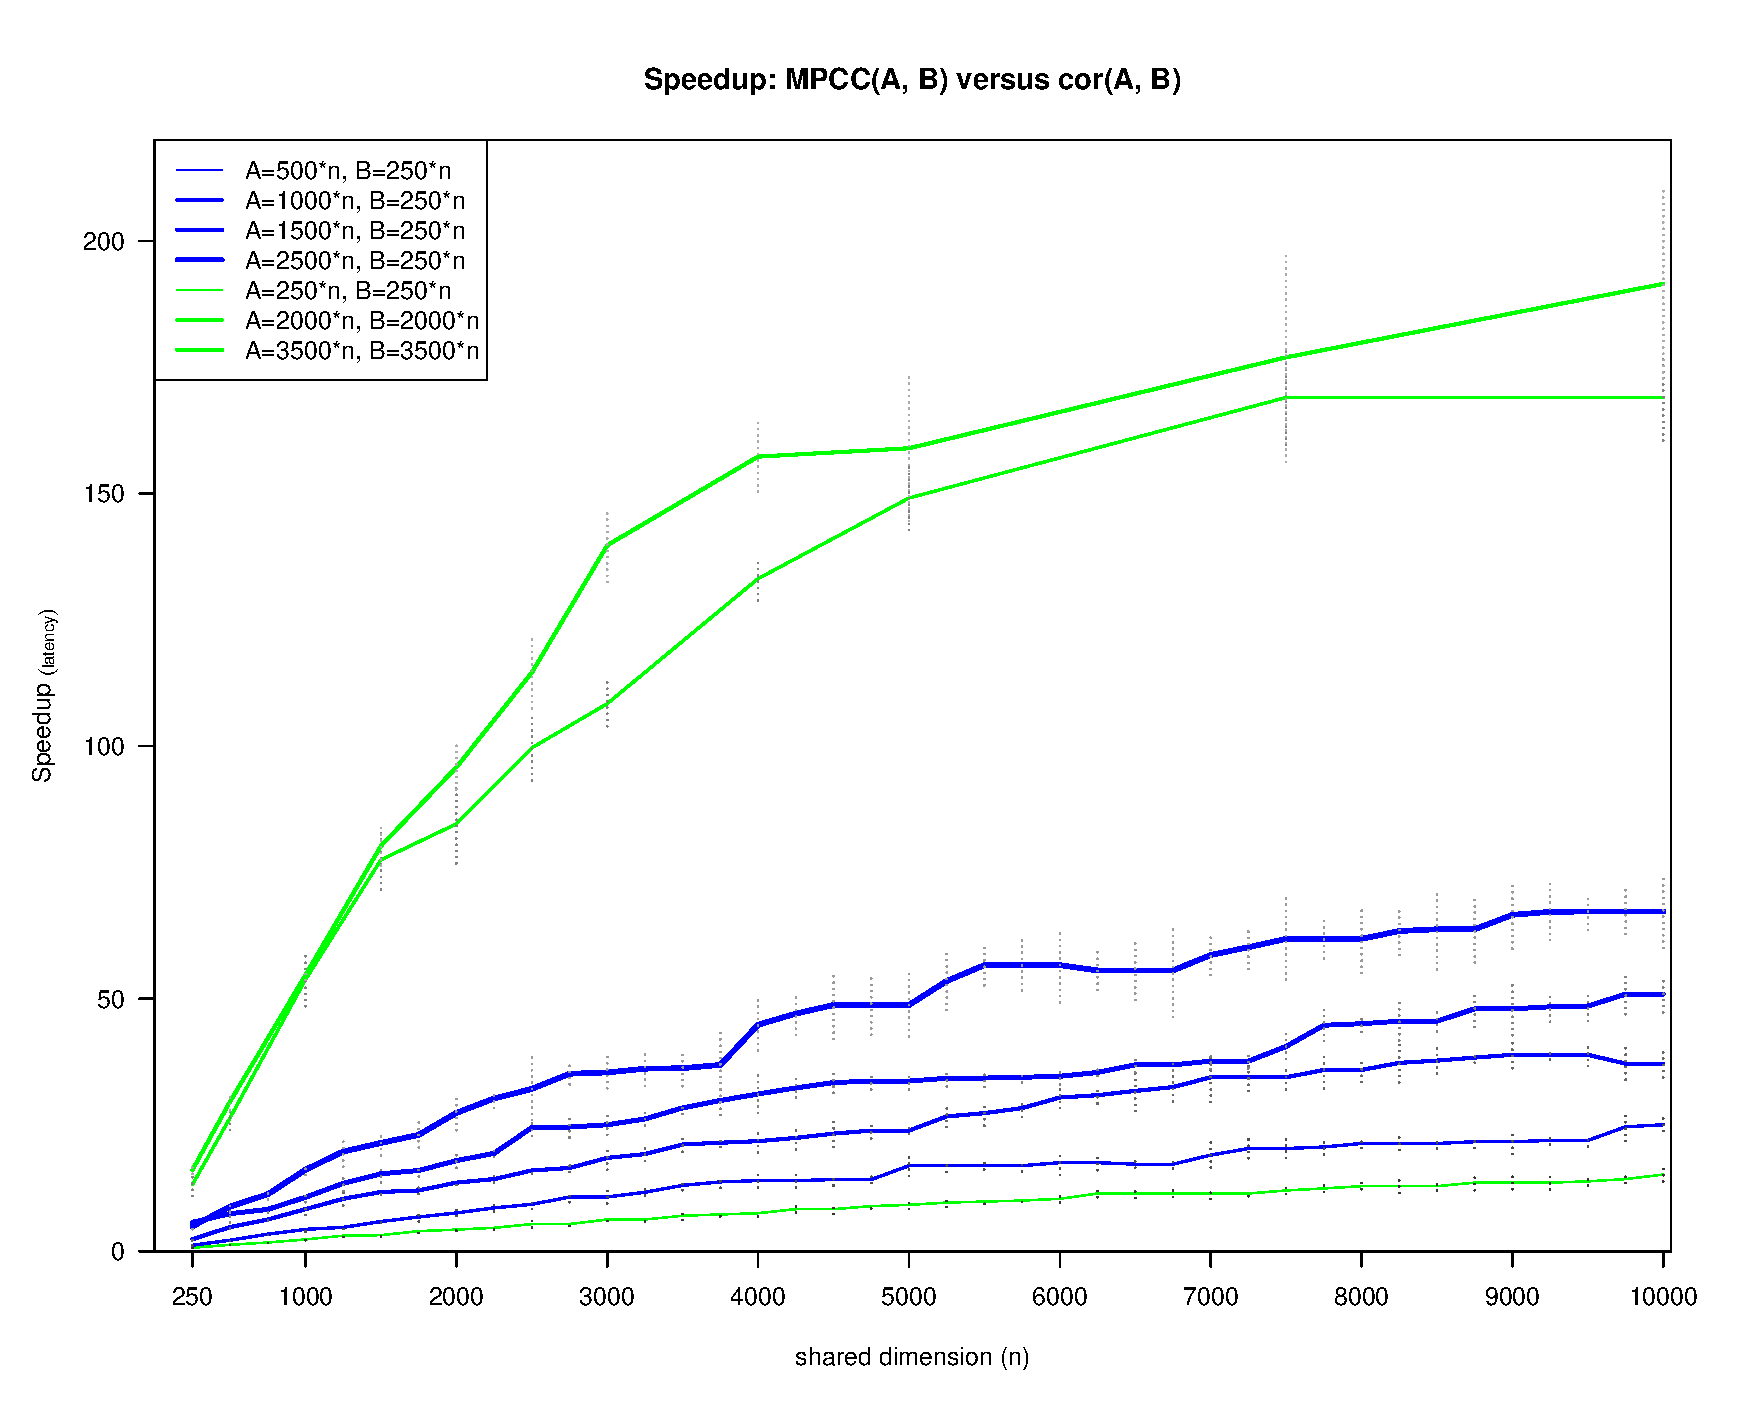
\includegraphics[width=\linewidth]{img/figure02new.eps}
  \caption{
  \small
    Speed comparison of MPCC versus the native R $cor$ function
    shows increased performance with growing matrix sizes. Increasing
    the amount of missing data (0 to 50\%), increased speedup compared 
    to the $cor()$ function. Since the missing data Bit-masking is always 
    performed, while the R $cor()$ function suffers from increased runtime 
    with increasing amount of missing data. Multi-threaded performance 
    of MPCC compared to the $cor()$ function showed a 200$\times$ speedup. 
    All timings were performed on a system with 28 cores (56 hyper threaded) Intel(R)
    Xeon(R) CPU E5-2680 v4 @ 2.40GHz.
}
  \label{fig:fig2}
\end{figure}

\vspace*{-5mm}

\section{Approach}

First we wrote a `naive' correlation function that is algorithmically
identical to the R $cor()$ function (see supplement). Multi-threading
support was added with little additional overhead by introducing
OpenMP. This naive version provided a multi-threaded baseline against
the full MPCC matrix version.  MPCC is a novel matrix implementation
of Pearson's correlation that makes use of hardware Advanced Vector
Extensions (AVX) instructions that were introduced by Intel in 2011.
The MPCC matrix version reformulates the original algorithm into a
series of matrix---matrix products and element-wise matrix
operations. MPCC handles missing data is by using a novel bit-masking
approach that leverages existing matrix---matrix multiplication
implementations from, for example, OpenBLAS (see supplement).

To benchmark MPCC for different matrix sizes we computed pairwise
correlation between genotypes of the BxD family.  Genotype data in the
BxD family is almost complete with only a few heterozygous or
`missing' loci remaining, i.e., this scenario benchmarks MPCC versus
$cor()$ when a small amount of data is missing.  Next we computed the
speed improvement of MPCC versus R's $cor()$ for these matrices. We
also increased step-wise the amount of missing data
(Figure \ref{fig:fig2}). Using MPCC on a single core to compute
genotype to genotype correlations showed a \textasciitilde{}5 times
reduction in runtime compared to the $cor()$ function provided in R.
Because the latter is not multi-threaded MPCC gains with every core
added, up to 200$\times$.  In comparison the naive version with OpenMP
to improve performance in comparison to the $cor()$ function provides
a consistent 3.5$\times$ speedup. This showed that the matrix---matrix 
multiplication implementation was responsible for the lion's share of 
performance gains, while the naive multi-threading support only marginaly 
improved performance.

% \vspace*{-5mm}
\section{Discussion}

Both the naive and Matrix versions provide R interfaces that act as
drop-in replacement for R's $cor()$ function.  MPCC leverages the
optimized speed of OpenBLAS or, alternatively, Intel\textregistered{}
MKL, to obtain maximum performance on systems that support the
AVX instruction sets.  The missing data
approach (Supplement 1 - 'Missing Data Bit-masking') can be trivially
generalized to other algorithms which rely on matrix---matrix
multiplication and may also be suitable for GPU computing.

While our work presents a reference implementation in R it is not
limited to the R programming language. MPCC is written in C and can
therefore be called from any other computer language using a foreign
function interface.

\section*{Funding}

We thank the support of Xsede/NSF startup MCB190140, the UT Center for
Integrative and Translational Genomics, and funds from the UT-ORNL
Governor's Chair, NIGMS Systems Genetics and Precision Medicine
Project R01 GM123489, NIDA grant P30 DA044223, NIAAA U01 AA013499 and
U01 AA016662.

\vspace*{-5mm}
\bibliographystyle{natbib}
\bibliography{main}

\end{document}
